%Eddy
\documentclass[a0paper,portrait]{baposter}
\usepackage[font=small,labelfont=bf]{caption} % Required for specifying captions to tables and figures
\usepackage{booktabs} % Horizontal rules in tables
\usepackage{relsize} % Used for making text smaller in some places
\usepackage{wrapfig} %Used to wrap images around text
\usepackage{xcolor}

\graphicspath{{figures/}} % Directory in which figures are stored

\definecolor{bordercol}{RGB}{255,214,51} % Border color of content boxes
\definecolor{headercol1}{RGB}{0,0,255} % Background color for the header in the content boxes (left side)
\definecolor{headercol2}{RGB}{0,0,10} % Background color for the header in the content boxes (right side)
\definecolor{headerfontcol}{RGB}{255,214,51} % Text color for the header text in the content boxes
\definecolor{boxcolor}{RGB}{186,215,230} % Background color for the content in the content boxes
\definecolor{textcol}{RGB}{255,255,255}%This is the color of text in textbox ajan just added this code and he is gassed

\begin{document}

\background{ % Set the background to an image (background.pdf)
\begin{tikzpicture}[remember picture,overlay]
\draw (current page.north west)+(-2em,2em) node[anchor=north west]
{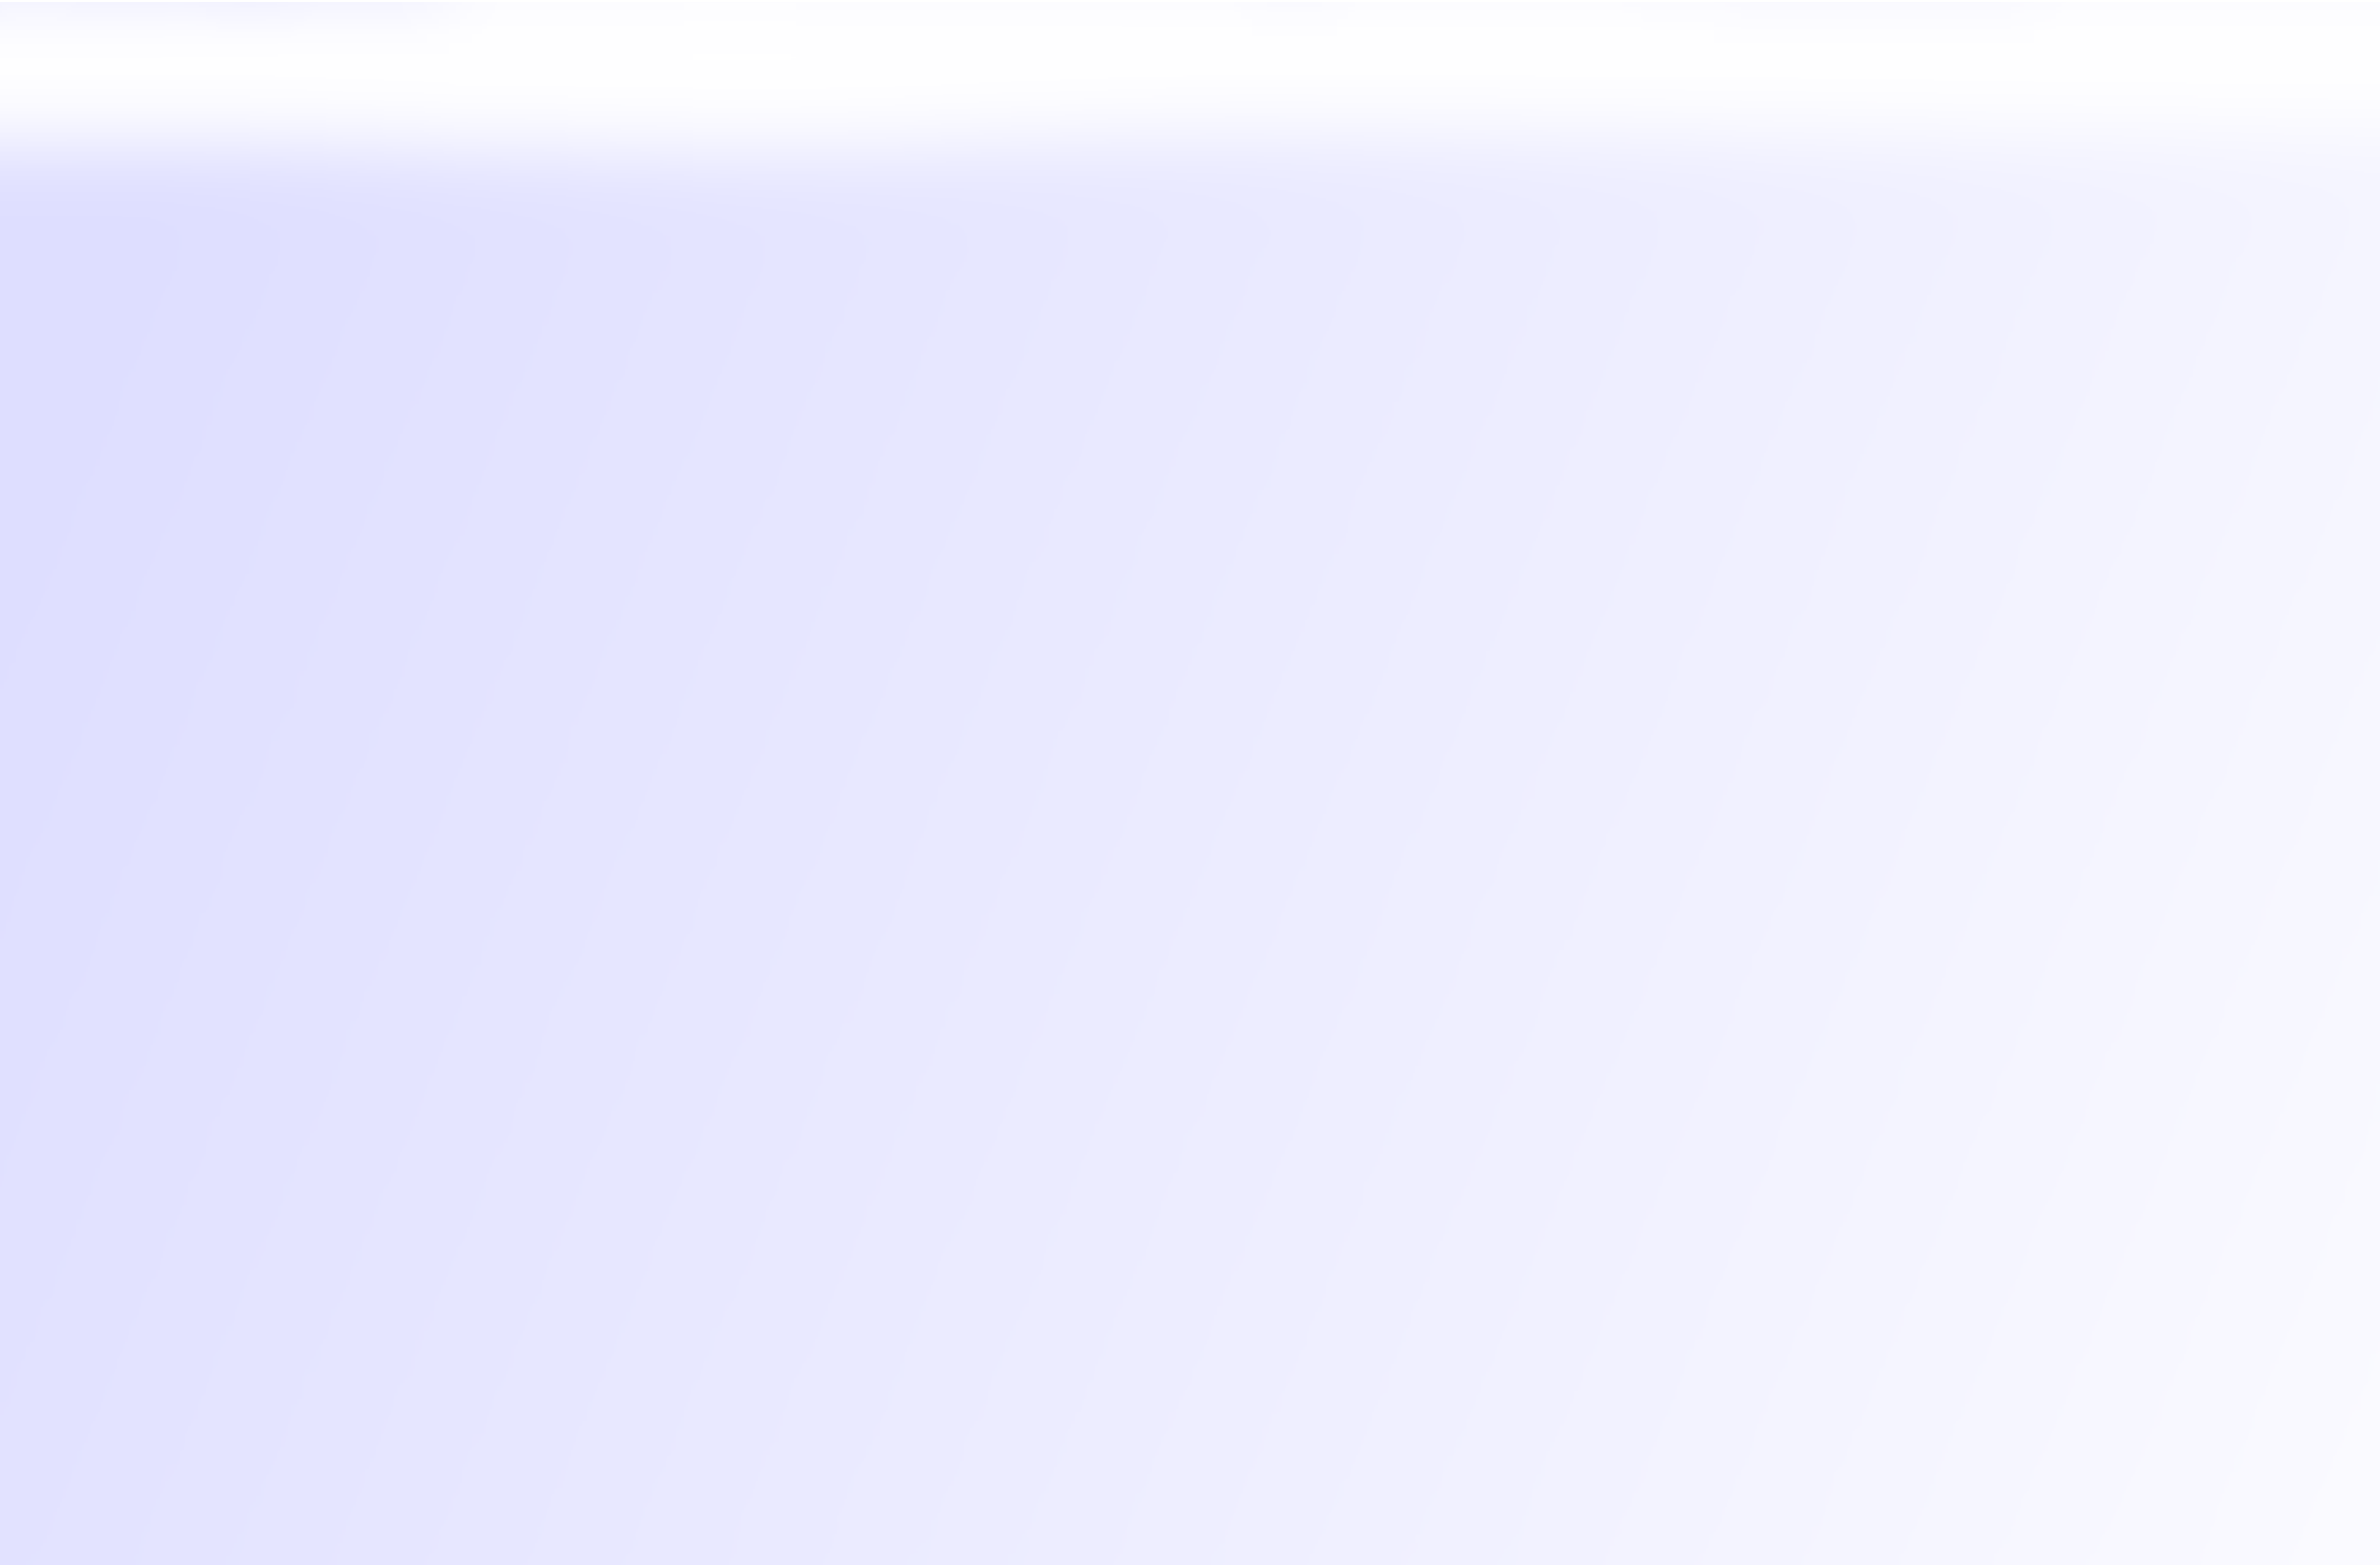
\includegraphics[height=1.1\textheight]{background}};
\end{tikzpicture}
}

\begin{poster}{
grid=false,
borderColor=bordercol, % Border color of content boxes
headerColorOne=headercol1, % Background color for the header in the content boxes (left side)
headerColorTwo=headercol2, % Background color for the header in the content boxes (right side)
headerFontColor=headerfontcol, % Text color for the header text in the content boxes
boxColorOne=boxcolor, % Background color for the content in the content boxes
headershape=roundedright, % Specify the rounded corner in the content box headers
headerfont=\Large\sf\bf, % Font modifiers for the text in the content box headers
textborder=rectangle,
background=user,
headerborder=open, % Change to closed for a line under the content box headers
boxshade=plain
}
{}
%----------------------------------------------------------------------------------------
%	TITLE AND AUTHOR NAME
%----------------------------------------------------------------------------------------
{\sf\bf The  Role  of  Electromagnetic  Radiation\\ in  Information  Communications} % Poster title
{\vspace{1em} Chris Wang, Eddy Tang, Ajan Manoharan, Lasse Lundberg, Alex Tiu, Kevin Teo\\The League of Eurasians || Blackett Laboratory, Imperial College London} % Author names
{
\includegraphics[scale=1.1]{the_logo}} % University/lab logo

%----------------------------------------------------------------------------------------
%	INTRODUCTION
%----------------------------------------------------------------------------------------

\headerbox{Introduction}{name=introduction,column=0,row=0}{
This poster outlines a variety of technologies, which use waves as a means to transfer information. These are both waves in the conventional sense of electromagnetic radiation, as well as the particle/wave duality sense of neutrinos.
}

%----------------------------------------------------------------------------------------
%	AFH
%----------------------------------------------------------------------------------------
\headerbox{Adaptive Frequency Hopping}{name=AFH,column=0,below=introduction}{
\textbf{What Is Frequency Hopping?} 
Adaptive Frequency Hopping (AFH) is a technique where rather than using a single radiofrequency to transfer data, the frequency is constantly changing between a number of channels. This allows for faster transfer speeds and makes it harder for intruders to interfere with the signal. 

\textbf{Why Is It Adaptive?} 
The transmitting device moniters different channels to estimate their quality. If one frequency is busy or being jammed, it will simply switch channels.
}

%----------------------------------------------------------------------------------------
%	Neutrinos
%----------------------------------------------------------------------------------------
\headerbox{Neutrino Messaging}{name=neutrino,column=0,below=AFH}{


A hypothetical form of communication that is currently undergoing research.
The presense and absense of neutrino pulses are represented as 1 and 0 respectively to encode messages. 
This was experimentally verified in 2012.\\
\textbf{Advantages}
Unlike traditional forms of communication which rely on electromagnetic radiation, neutrinos are
affected only by the weak force and gravity; they can pass messages through virtually
anything.
This can be utilised to transmit information across vast expanses in space, or for a more present-day application,
to send messages to nuclear submarines, as seawater can obstruct
electromagnetic radiation.\\
\textbf{Disadvantages}
The uninteractive nature of neutrinos causes them to be difficult to detect. Neutrinos also oscillate
between 3 flavours - electron, muon, and tau. This can be represented by a neutrino switching
between waves of different frequencies as it travels through space, which can be a problem for detection.

}


%----------------------------------------------------------------------------------------
%	CONCLUSION
%----------------------------------------------------------------------------------------

\headerbox{Conclusion}{name=conclusion,column=0,below=neutrino}{
These technologies have changed the world, allowing us to be interconnected to a much greater extent than any time before. Many people's livelihoods, and some of the largest industries on the planet, revolve around wave-based communication. In the future, neutrino messaging may solve electromagnetic radiation-based communication's range and interference issues. 
}

%----------------------------------------------------------------------------------------
%	REFERENCES
%----------------------------------------------------------------------------------------

\headerbox{References}{name=references,column=0,below=conclusion,above=bottom}{

\smaller % Reduce the font size in this block
\renewcommand{\section}[2]{\vskip 0.05em} % Get rid of the default "References" section title
\nocite{*} % Insert publications even if they are not cited in the poster

\bibliographystyle{unsrt}
\bibliography{references} % Use sample.bib as the bibliography file
}

%----------------------------------------------------------------------------------------
%	Wi-Fi
%----------------------------------------------------------------------------------------
\headerbox{Wi-Fi}{name=wifi,span=2,column=1,row=0}{ % To reduce this block to 1 column width, remove 'span=2' 

Wi-Fi is defined as any “wireless local area network (WLAN) products that are based on the IEEE 802.11 standards." It is usually a wave of frequency between 2.4GHz to 5GHz. Networks are created through Wi-Fi where multiple devices can connect to one source of Wi-Fi and thus access the internet as well as communicate with other devices connected to the network.  \linebreak

\textbf{Advantages}\\
•	Remote access for convenience\\
•	Can support multiple simultaneous connections\\
• 	Uses AFH, as explained on the left side of this poster

\textbf{Disadvantages}\\
•	Limited by router location\\
•	Subject to interference\\
•	Slow speed compared to wired connections
}

%----------------------------------------------------------------------------------------
%	Optical Fibres
%----------------------------------------------------------------------------------------
\headerbox{Optical Fibres}{name=optical_fibre,span=2,column=1,below=wifi}{

Optical fibres utilise total internal reflection to confine light rays within its core. Modern fibre technologies are limited by physical phenomena of light travelling in an optical medium. \\

\textbf{Residual Absorption}
Fundamental vibration frequencies of the particles that make up the glass absorbs light of matching frequencies.   

\textbf {Dispersion}
An optical phenomenon that causes light of different wavelengths to travel at different velocities through an optical medium. This creates a disparity in the time of a single pulse of light at the receving end, which can corrupt the transferred data



\textbf {Rayleigh Scattering}
An atom or molecule reradiates incident light in any direction except the incident direction.

}

%----------------------------------------------------------------------------------------
%	Bluetooth
%----------------------------------------------------------------------------------------
\headerbox{Bluetooth {
\includegraphics[scale=0.02]{bluetooth_logo}}}{name=bluetooth,span=2,column=1,below=optical_fibre}{

\begin{wrapfigure}{r}{0.25\textwidth}
	{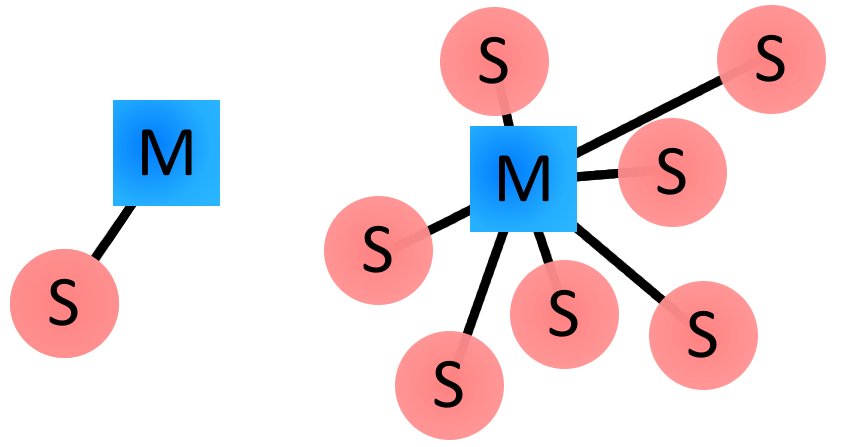
\includegraphics[scale=0.12]{master_slave_topology}} % University/lab logo
\end{wrapfigure}

Bluetooth was developed by the Swedish telephone company Ericsson AB in 1990 \\

\textbf{Master/Slave Topology}
Bluetooth follows a master/slave topology where there is a master device broadcasting data to a maximum of seven slave devices. This network of 8 devices is
known as a piconet. The master will always default to being the device which
initialised the connection. However, master and slave roles can be exchanged
given that both devices agree upon this. 


\textbf{AFH}
Bluetooth uses a technique known as AFH, which is explained on the left side of this poster.
}

%----------------------------------------------------------------------------------------
%	Li-Fi
%----------------------------------------------------------------------------------------
\headerbox{Li-Fi}{name=lifi,span=2,column=1,below=bluetooth}{



%\begin{wrapfigure}{r}{0.26\textwidth}
%	{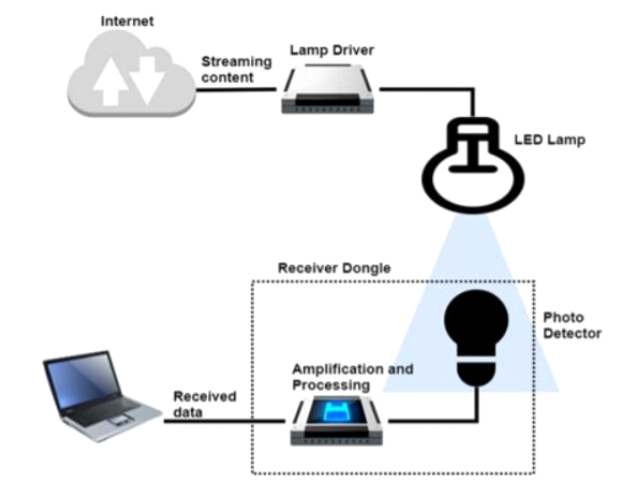
\includegraphics[scale=0.17]{Lifi}}
%\end{wrapfigure}               

Li-Fi involves the use of light emitters that modulate light intensity and a photo detector that receives the signal and converts it back into an electrical data stream. \linebreak

%A light emitter, a photo detector; Modulate light intensity faster than eyes can follow; Receiver dongle converts  changes electrical signals; Signals converted back into a data stream and transferred to a mobile device.
                                   
                              
 \textbf{Advantages} \\
• High bandwidth compared to mobile signals \\
• Minimal maintenance and setup costs 

\textbf{Disadvantages}\\
• Can be obstructed easily\\
• Prone to interference from other light sources \\
• Limited to point-to-point transfer at very high frequencies.


}

%----------------------------------------------------------------------------------------
%	NFC
%----------------------------------------------------------------------------------------
\headerbox{Near Field Communication}{name=nfc,span=2,column=1,below=lifi, above=bottom}{

Near Field Communication (NFC) uses small chips to enable data transfer between active and passive devices. Active devices are powered externally and can both send and receive data. Passive devices do not require a power source and can only send data. In close proximity, active devices will induce small currents in passive ones. \linebreak

\begin{wrapfigure}{r}{0.325\textwidth}
	{\includegraphics[scale=0.195]{NFC_Diagram}}
\end{wrapfigure}


\textbf{Stats}\\
• Max Range = 20cm\\ 
• Max Speed = 424kbit/s\\
• Transmission Frequency = 13.56MHz

\textbf{Advantages}\\
• Power Efficiency\\
• Control and Security\\
• Convenience

\textbf{Disadvantages}\\
• Low transfer speed

}


\end{poster}

\end{document}